\section{Proposed Method}
\label{methods}
The goal of this study is to classify \ac{rcm} images according to 3 labels (Malignant, Benign and Healthy) firstly using two schemes, namely using the whole image and using the local or patch-based approach. The feature extraction is common to both schemes, we therefore start by describing it in the next Section before presenting the different ways we propose to combine local information to build final decision.\par

\subsection{Feature Extractors}
\label{descriptors}
The first extractor is based on Daubechies wavelets along three axes: horizontal, vertical and diagonals as suggested by an article~\cite{Halimi2017a}. Extraction of wavelets is performed by using “PyWavelet” library~\cite{lee2006pywavelets}. Then reduction of the number of parameters is achieved to avoid data over-fitting and time-consuming computation. Extracted coefficients are reduced using Generalized Gaussian Distribution by keeping only $\alpha$ and $\beta$ coefficients, respectively the scale and shape parameters of this distribution. To ease the readability, we will call this method “Wavelets”.\par
The second feature extractor is using Haralick~\cite{Haralick1973} as input information for classifier. These characteristics are extracted along four axes: horizontal, vertical and two diagonals. These are statistical-based descriptors, efficient in describing pattern on textured images. Haralick features are extracted using “Mahotas” library~\cite{coelho2012mahotas}. For the sake of clarity, we will call this method “Haralick” in the remainder of this paper.\par
The last feature extractor is based on pretrained \acsp{cnn}, which are known to be well-suited methods for image classification, thanks to robust feature patterns. Our work focuses on Google “InceptionV3” architecture~\cite{Szegedy2015} as it is supposed to perform well on medical images according to recent studies~\cite{Litjens2017}. Instead of training this network from scratch, we choose a Transfer Learning approach (originally trained on ImageNet database~\cite{Deng2008}) which is appropriate for a problem similar to the original database and when the amount of data is reduced. In order to get this new representation of data, we removed the last layers devoted to classification. Furthermore, in order to reduce the number of features provided by the \acsp{cnn}, we use and compare two pooling techniques on spatial dimension based on maximum and average value. Implementation is made with “Keras” library~\cite{chollet2015keras}. For convenience, this whole method will be called “Transfer Learning”, and we will use respectively “Max Pool” and “Avg Pool” to make reference to maximum and average pooling layers in the next paragraphs.\par
\subsection{Presentation of pipelines}
\label{pipelines}
We designed two processing pipelines corresponding to the two approaches we propose and aim to compare: i) classification using the entire image and ii) local or patch-based classification and merging. The first pipeline gives us clues regarding the selection of the most appropriate feature extractor, that we can use later locally (patch) within the second pipeline. In both cases, the extracted features are always normalized, based on a standard score computation to make classification task more accurate and robust. This scaling is computed by subtracting the mean value, and then dividing by standard deviation value.\par
Finally, a classification task is performed by a classical linear SVM. As our goal is to evaluate the most relevant features related to our \ac{rcm} images, we make use of a simple linear kernel. The first processing pipeline is illustrated in \Cref{simple}.\par
\begin{figure}[H]
    \begin{center}
        \includegraphics[width=0.65\linewidth]{content/figures/Simple.pdf}
        \caption{Pipeline for classification of \ac{rcm} images.}
        \label{simple}
    \end{center} 
\end{figure}
As we want to understand how local areas within an image contribute to the final decision, we designed a second processing pipeline. The difference with the first one is that we operate a training and classifications on patches that we merge to make the final decision on the whole image. This kind of approach was suggested by recent researches on histology images by~\cite{Xu2015,Hou2016}. In our implementation however, instead of using a prediction on the whole image as they do, we carry out both training and prediction on patches. Local predictions provide scores or decisions used to train a linear SVM at higher level along same classes, and provide respectively a decision called “Score level” or “Decision level”. This processing pipeline is illustrated in \Cref{sliding}.\par
\begin{figure}[h]
    \begin{center}
        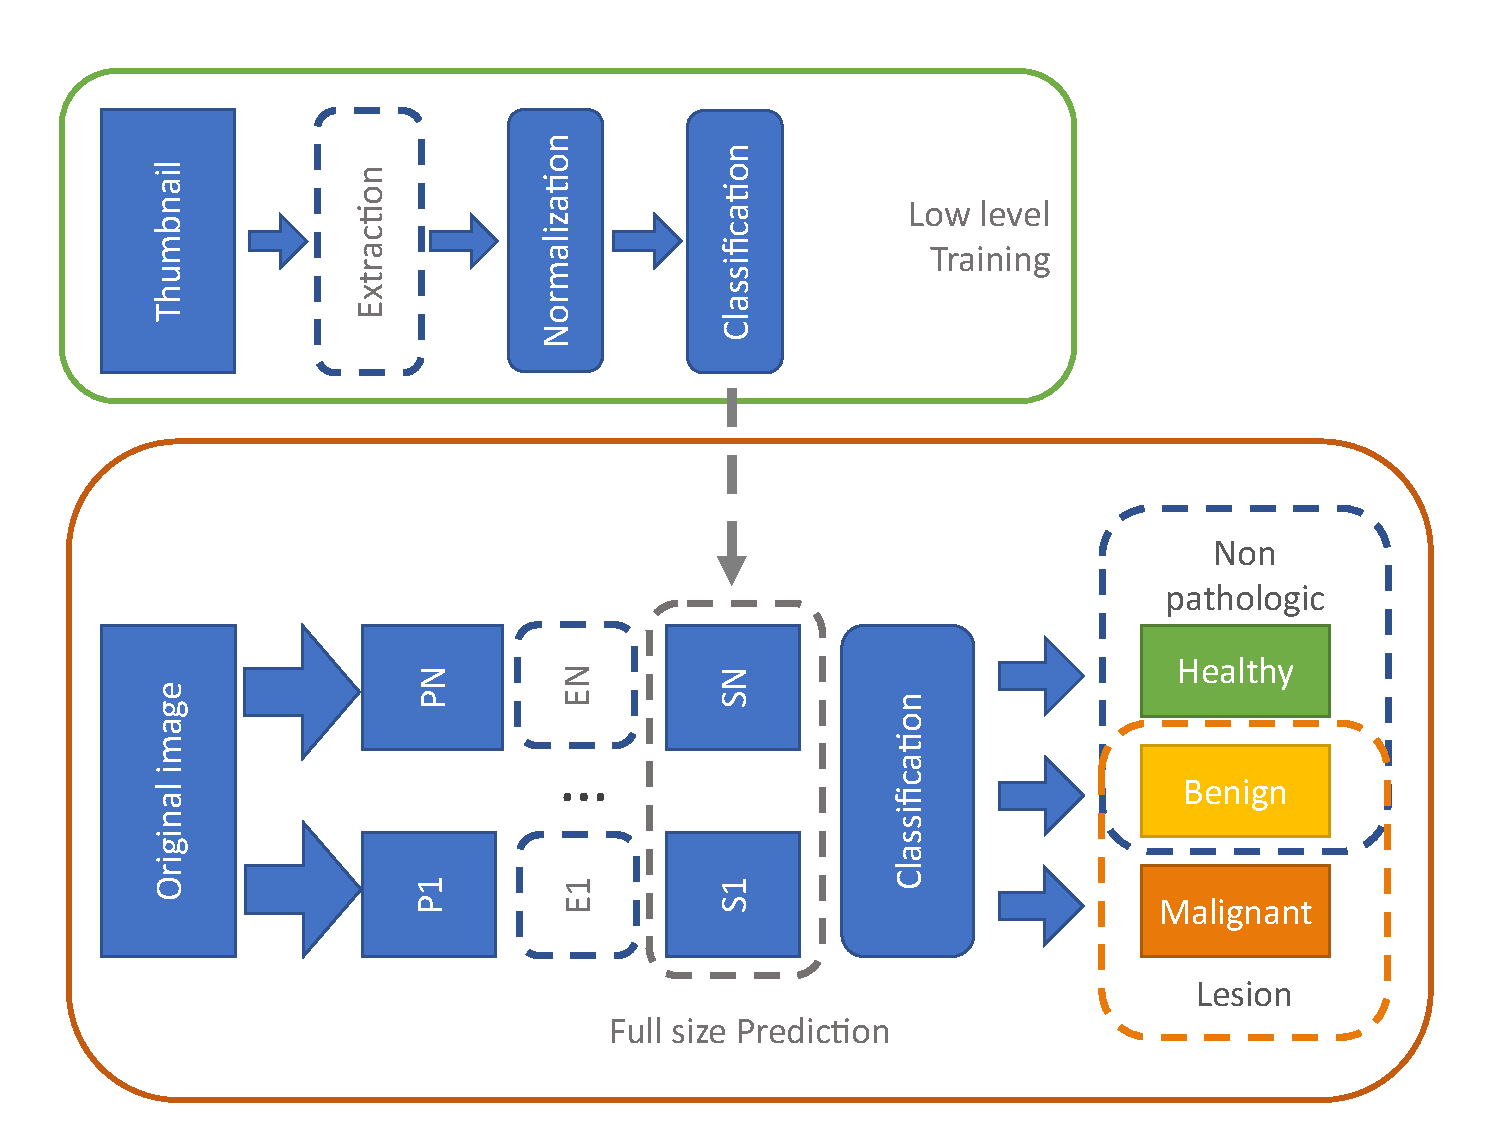
\includegraphics[width=0.65\linewidth]{content/figures/Sliding.pdf}
        \caption{Second pipeline for classification \ac{rcm} images. P1 to PN correspond to Patches, E1 to EN correspond to feature Extraction and S1 to SN correspond to Scores or Decisions obtained for each patches.}
        \label{sliding}
    \end{center} 
\end{figure}